\documentclass{standalone}
\usepackage{tikz}
\usetikzlibrary{patterns}
\usetikzlibrary{positioning}
\usetikzlibrary{patterns, positioning}
\usetikzlibrary{shapes.misc}
\usepackage[outline]{contour}
\contourlength{1.5pt} 


\begin{document}
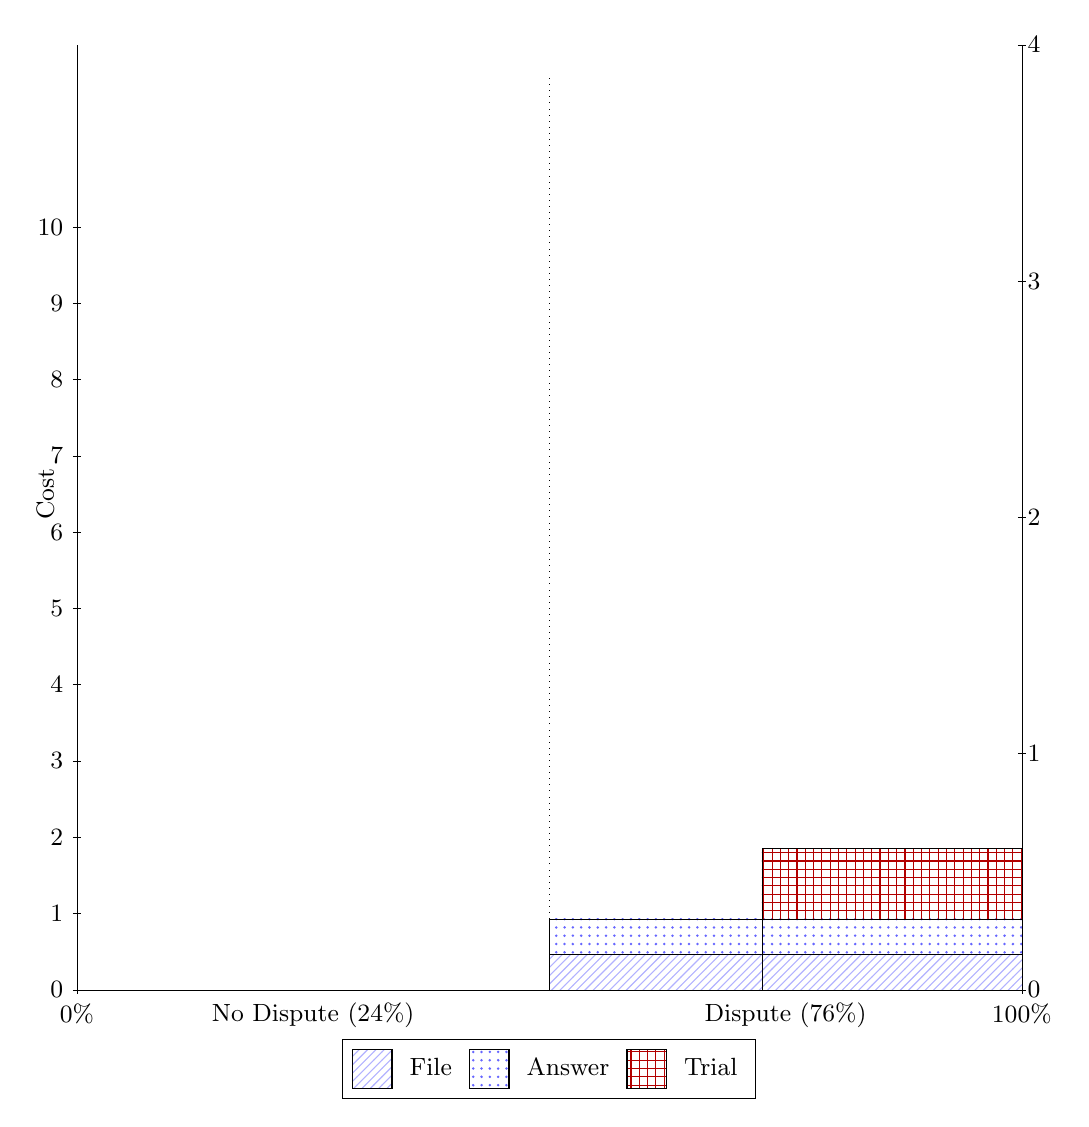
\begin{tikzpicture}
\draw[pattern=north east lines, pattern color=blue!30,draw=black,very thin] (7.5,2.5) rectangle (10.198,2.95);
\draw[pattern=dots,  pattern color=blue!60,draw=black,very thin] (7.5,2.95) rectangle (10.198,3.4);
\draw[pattern=north east lines, pattern color=blue!30,draw=black,very thin] (10.198,2.5) rectangle (13.5,2.95);
\draw[pattern=dots,  pattern color=blue!60,draw=black,very thin] (10.198,2.95) rectangle (13.5,3.4);
\draw[pattern=grid,            pattern color=red!70!black,draw=black,very thin] (10.198,3.4) rectangle (13.5,4.3);
\draw[black,very thin] (1.5,2.5) -- (1.5,14.5);
\node[font=\small,rotate=90,text=black, anchor=center] at (1.1, 8.7967) {Cost};
\draw[black,very thin] (1.45,2.5) -- (1.55,2.5);
\node[font=\small,text=black, anchor=east] at (1.45, 2.5) {0};
\draw[black,very thin] (1.45,3.4687) -- (1.55,3.4687);
\node[font=\small,text=black, anchor=east] at (1.45, 3.4687) {1};
\draw[black,very thin] (1.45,4.4375) -- (1.55,4.4375);
\node[font=\small,text=black, anchor=east] at (1.45, 4.4375) {2};
\draw[black,very thin] (1.45,5.4062) -- (1.55,5.4062);
\node[font=\small,text=black, anchor=east] at (1.45, 5.4062) {3};
\draw[black,very thin] (1.45,6.3749) -- (1.55,6.3749);
\node[font=\small,text=black, anchor=east] at (1.45, 6.3749) {4};
\draw[black,very thin] (1.45,7.3436) -- (1.55,7.3436);
\node[font=\small,text=black, anchor=east] at (1.45, 7.3436) {5};
\draw[black,very thin] (1.45,8.3124) -- (1.55,8.3124);
\node[font=\small,text=black, anchor=east] at (1.45, 8.3124) {6};
\draw[black,very thin] (1.45,9.2811) -- (1.55,9.2811);
\node[font=\small,text=black, anchor=east] at (1.45, 9.2811) {7};
\draw[black,very thin] (1.45,10.25) -- (1.55,10.25);
\node[font=\small,text=black, anchor=east] at (1.45, 10.25) {8};
\draw[black,very thin] (1.45,11.219) -- (1.55,11.219);
\node[font=\small,text=black, anchor=east] at (1.45, 11.219) {9};
\draw[black,very thin] (1.45,12.187) -- (1.55,12.187);
\node[font=\small,text=black, anchor=east] at (1.45, 12.187) {10};

\draw[black,dotted,very thin] (7.5,2.86) -- (7.5,14.14);
\draw[black,very thin] (13.5,2.5) -- (13.5,14.5);
\draw[black,very thin] (13.45,2.5) -- (13.55,2.5);
\node[font=\small,text=black, anchor=west] at (13.45, 2.5) {0};
\draw[black,very thin] (13.45,5.5) -- (13.55,5.5);
\node[font=\small,text=black, anchor=west] at (13.45, 5.5) {1};
\draw[black,very thin] (13.45,8.5) -- (13.55,8.5);
\node[font=\small,text=black, anchor=west] at (13.45, 8.5) {2};
\draw[black,very thin] (13.45,11.5) -- (13.55,11.5);
\node[font=\small,text=black, anchor=west] at (13.45, 11.5) {3};
\draw[black,very thin] (13.45,14.5) -- (13.55,14.5);
\node[font=\small,text=black, anchor=west] at (13.45, 14.5) {4};

\draw[black,very thin] (1.5,2.5) -- (13.5,2.5);
\draw[black,very thin] (1.5,2.45) -- (1.5,2.55);
\node[font=\small,text=black, anchor=north] at (1.5, 2.45) {0\%};
\draw[black,very thin] (13.5,2.45) -- (13.5,2.55);
\node[font=\small,text=black, anchor=north] at (13.5, 2.45) {100\%};

\node[font=\small,text=black,anchor=south] at (4.5, 1.9) {No\ Dispute\ (24\%)};
\node[font=\small,text=black,anchor=south] at (10.5, 1.9) {Dispute\ (76\%)};
\draw (7.5,2.5) node (B) {};
\begin{scope}[align=center]
\matrix[scale=0.5,draw=black,below=0.5cm of B,nodes={draw},column sep=0.1cm]{
\node[rectangle,draw,minimum width=0.5cm,minimum height=0.5cm,pattern=north east lines, pattern color=blue!30]{}; & \node[draw=none,font=\small,text=black]{File}; &
\node[rectangle,draw,minimum width=0.5cm,minimum height=0.5cm,pattern=dots,  pattern color=blue!60]{}; & \node[draw=none,font=\small,text=black]{Answer}; &
\node[rectangle,draw,minimum width=0.5cm,minimum height=0.5cm,pattern=grid,            pattern color=red!70!black]{}; & \node[draw=none,font=\small,text=black]{Trial}; \\\\
};\end{scope}

\end{tikzpicture}
\end{document}